\section{Methoden}
	
	Dieser Abschnitt befasst sich mit dem Aufbau des Franck-Hertz-Versuches, so wie auch den dabei auftretenden Unsicherheiten.
	
	\subsection{Aufbau}		
		\begin{figure}[ht]
			\centering
			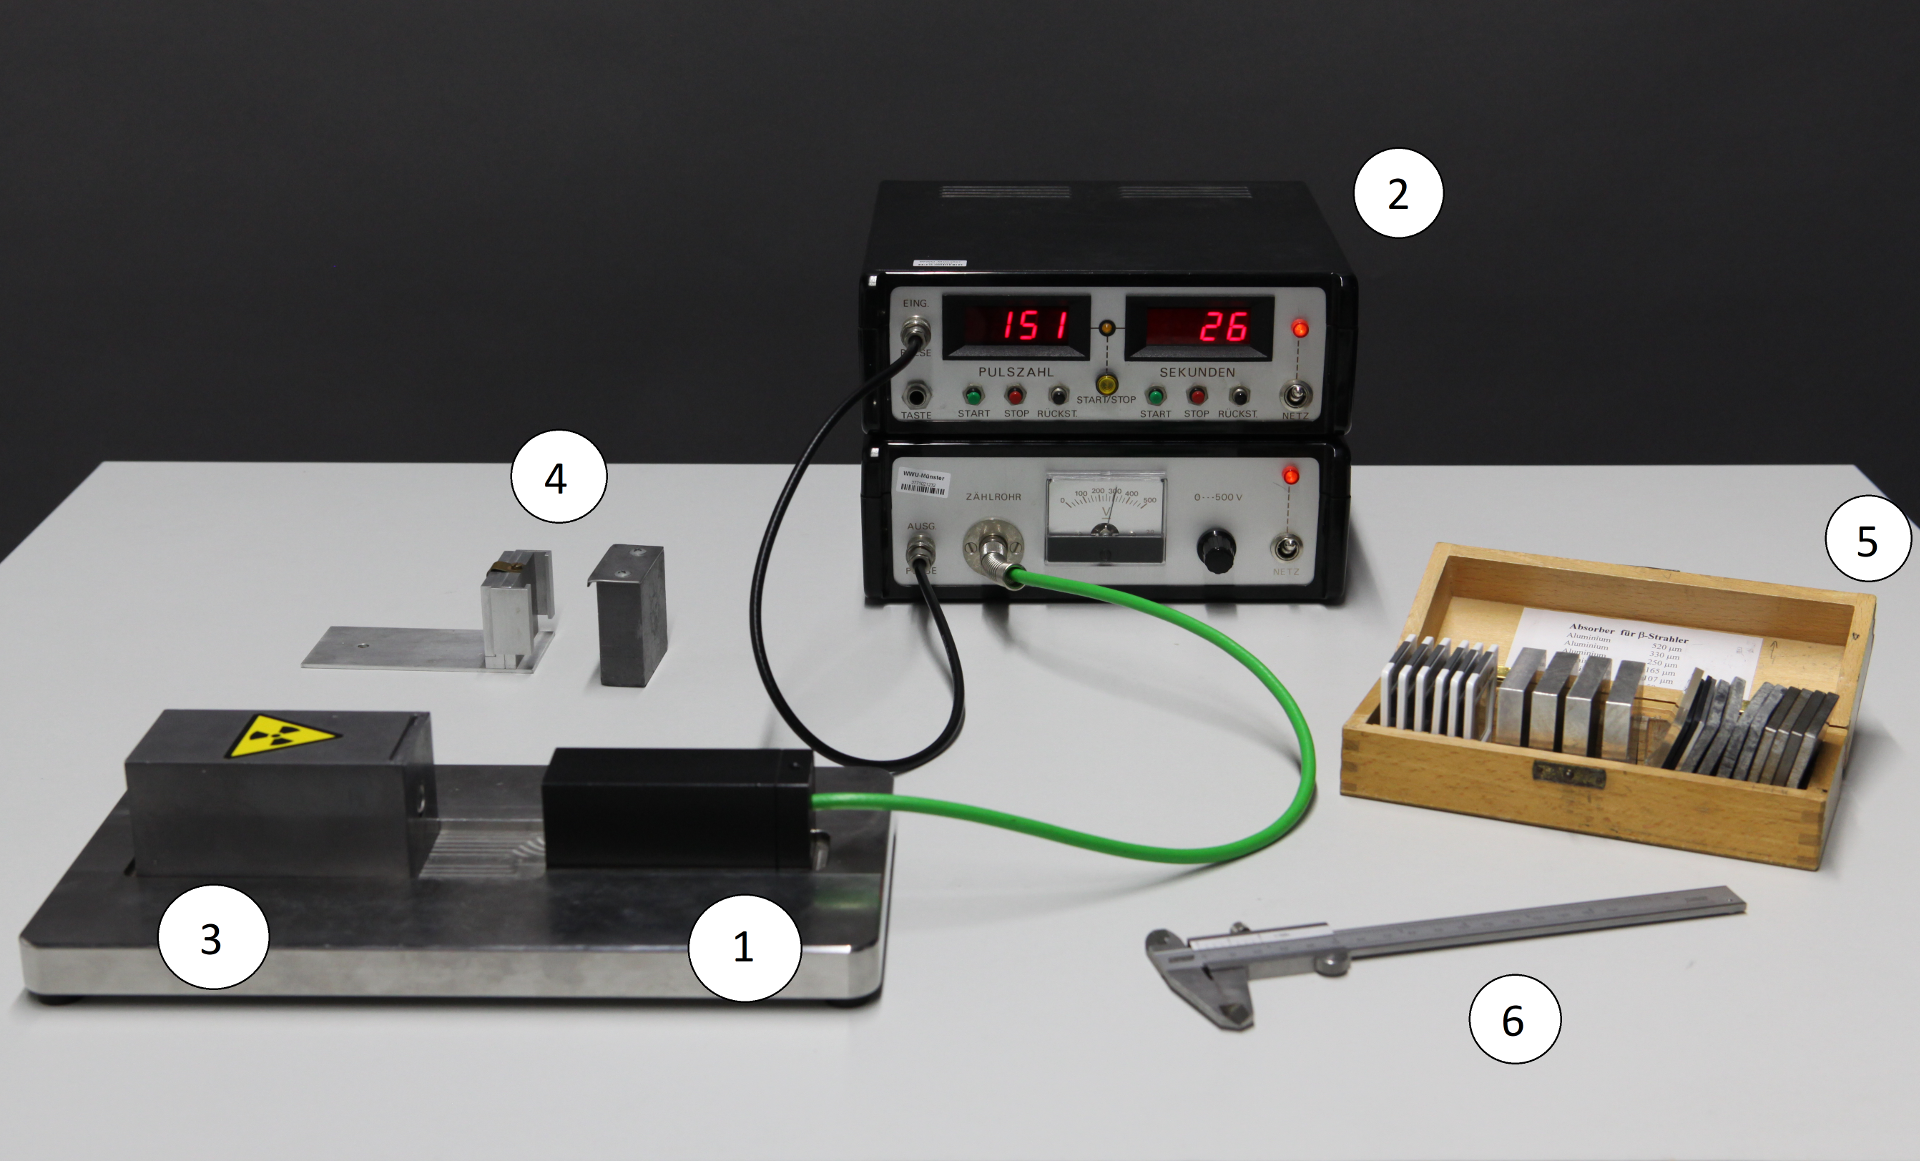
\includegraphics[width=\textwidth]{bilder/Aufbau.png}
			\caption{Diese Abbildung stellt die Schaltung der Franck-Hertz-Röhren (Hg links, Ne rechts) dar. \cite{WWU}}
			\label{fig:Aufbau}	
		\end{figure}	
		Wie in Abbildung \ref{fig:Aufbau} dargestellt, besteht der Aufbau des Franck-Hertz-Versuches im Wesentlichen aus einer Triode, welche mit einem Neongas bzw. flüssigem Quecksilber gefüllt ist. 
		Aus der Kathode werden Elektronen ausgesandt und zur Anode geschickt.		
		Vor dem Gitter, welches zwischen Kathode und Anode liegt, werden diese mit der Beschleunigungsspannung	$U_B$ beschleunigt und hinter dem Gitter mit der Gegenspannung $U_G$ abgebremst.
		Bei der Neonröhre ist hinter der Kathode zusätzlich ein Steuergitter, um die Elektronen mit der Spannung $U_S$ für den Versuch besser zu verteilen.
		Da der elektrische Strom an der Anode sehr gering ist, wird stattdessen die eingehende Spannung gemessen, da diese bei diesem Aufbau proportional zu dem Strom ist.
		Für das Quecksilber werden zwei Messungen durchgeführt.
		Einmal bei Zimmertemperatur, im flüssigem Zustand und dann als Gas. 
		Damit der gasförmige Zustand erreicht werden kann, befindet sich die Quecksilberröhre in einem Ofen, der für die zweite Messung auf ca. $\SI{200}{\celsius}$ erhitzt wird.
		Ein hoher Druck ist notwendig um eine Reihe von Elektronenstößen an den Atomen zu ermöglichen.
		
	\subsection{Unsicherheiten} 
	
		Bei diesem Versuch treten die Unsicherheiten primär bei den Digitalanzeigen der Messgeräte für Spannung und Temperatur auf. 
		Die Gegenspannung wird analog eingestellt und erhält eine Unsicherheit von %TODO.
		Die Berechnung der kombinierten Unsicherheiten erfolgt nach GUM und ist im Anhang aufgeführt.

\section{Durchführung und Datenanalyse}
	
	Vor der Aufnahme der Messungen wurde der Aufbau an ein Oszilloskop geschlossen, um den Verlauf der Franck-Hertz-Kurven zu verbildlichen (siehe Abb. \ref{label} im Anhang). 
	Für eine optimale Aufnahme der $I_A/U_B$-Charakteristiken wurde mit Hilfe des Oszilloskop die Gegenspannung $U_G$ gesucht, bei der die Charakteristiken am deutlichsten erkennbar war.
	Diese Gegenspannung lag bei $\approx \SI{1}{\volt}$.
	
	Während der Aufnahme der Werte war bei der Neonröhre ein rötliches Leuchten zu erkennen, welches mit steigender Beschleunigungsspannung $U_B$ intensiver wurde.  
	Bei dem Quecksilber war bei den beiden Messungen keine solche Beobachtung möglich.
	
	\begin{figure}[ht]
		\centering
		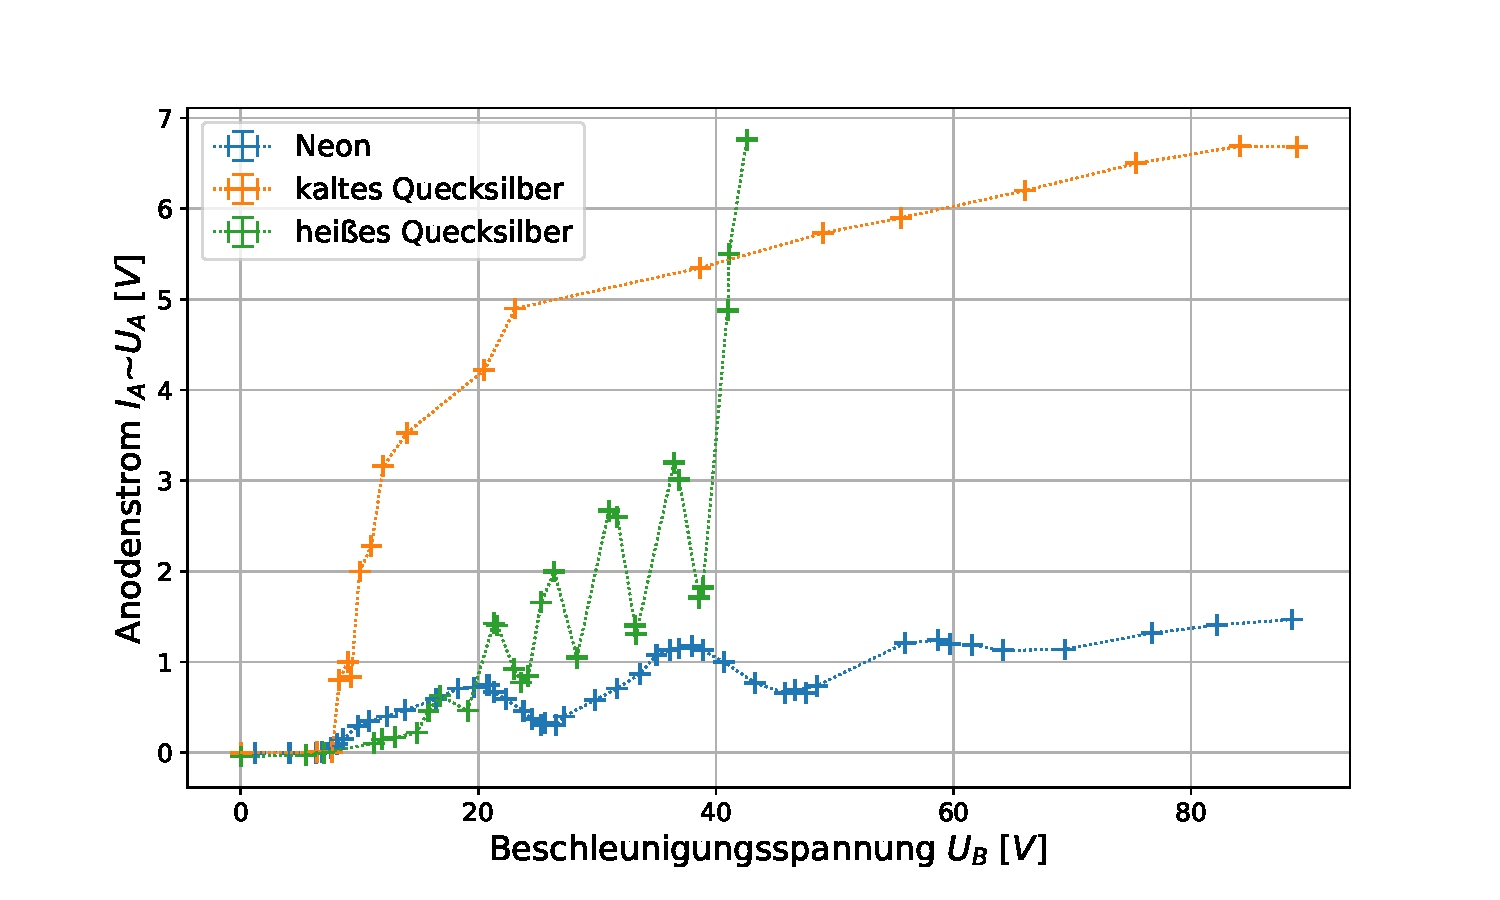
\includegraphics[width=\textwidth]{data/CharakteristikZusammen.pdf}
		\caption{Diese Abbildung stellt die $I_A/U_B$-Charakteristiken graphisch dar.}
		\label{fig:Kurve}	
	\end{figure}
	Die aufgenommen Werte für die $I_A/U_B$-Charakteristiken sind in Abbildung \ref{fig:Kurve} dargestellt. 
	Zu erkennen ist bereits, dass der Kurvenverlauf bei dem flüssigem Quecksilber der Kennlinie einen logarithmischen Verlauf annimmt, wohingegen bei dem Neon und noch ausgeprägter bei dem erhitzten Quecksilber der gemessene Anodenstrom wiederholt zu- und abnimmt, so dass ein "zackiges" Muster entsteht.\footnote{Die Linien zwischen den Messwerten dienen nur zur Verbildlichung und entsprechen nur genähert dem beobachteten Spannungsverlauf}. 
	Bei dem heißen Quecksilber sind fünf Maxima erkennbar, bei dem Neon hingegen drei.
	
	Mit Hilfe dieser Messungen lassen sich über die Minima (oder wie hier die Maxima) die Energien der Elektronen bestimmen, die nötig sind um die Atome der Gase anzuregen.
	Dazu dient $E=eU$. 
	
	Bei dem Zurückfallen eines angeregten Atoms in den Ruhezustand wird Licht emittiert. 
	Dieses hat je nachdem von welchem Zustand zurückgefallen wird eine andere Wellenlänge. 
	Über $\lambda = \frac{h \cdot c}{E}$ lässt sich diese Wellenlänge berechnen.
	Dabei ist $h$ das planck'sche Wirkungsquantum.
	Zudem lässt sich über die Wellenlänge auch die Frequenz des emittierten Lichts über $f = \frac{c}{\lambda}$ ermitteln. 
	In Tabelle \ref{tab:Werte} sind die Energien bei den verschiedenen Maxima, an denen die Anregung der Atome stattfindet, sowie auch die Frequenzen und Wellenlängen, welche dem darauf emittierten Licht zugehören, verzeichnet.
	\begin{table}
		\caption{In dieser Tabelle sind die ermittelten Energien, Wellenlängen und Frequenzen dargestellt.}
		\label{tab:Werte}
		\centering
		\begin{tabular}{c|c|c|c|c}
			& Max. & E & $\lambda$ & $f$ \\			
			\hline		
			Ne 	& 1. & & & \\
				& 2. & & & \\
				& 3. & & & \\
			\hline
			Hg(g) 	& 1. & & & \\
					& 2. & & & \\
					& 3. & & & \\
					& 4. & & & \\
					& 5. & & & \\					
		\end{tabular}
	\end{table}

	Zur Bestimmung des Dampfdrucks in der Quecksilberröhre dient die Clausius-Clapeyron Formel (\ref{eq:Clausius}):
	\begin{align} \label{eq:Clausius}
		a = b	%TODO Formel
	\end{align}
	Mit Hilfe des dadurch ermittelten Drucks lässt sich nun die freie Weglänge der Elektronen in dem Quecksilbergas berechnen. 
	Diese wird durch Gleichung \ref{eq:Weg} beschrieben:
	\begin{align} \label{eq:Weg}
		\lambda_\text{frei} = \frac{k_\text{B}\cdot T}{\sigma\cdot p}.
	\end{align}
 	Einsetzen mit $\sigma = \pi R^2$ und $T = \SI{192+-2}{\celsius}$ liefert eine freie Weglänge $\lambda_\text{frei} =$. %TODO Wert und Unsicherheit Temperatur korrigieren

\section{Diskussion}
	
	\begin{figure}[ht]
		\centering
		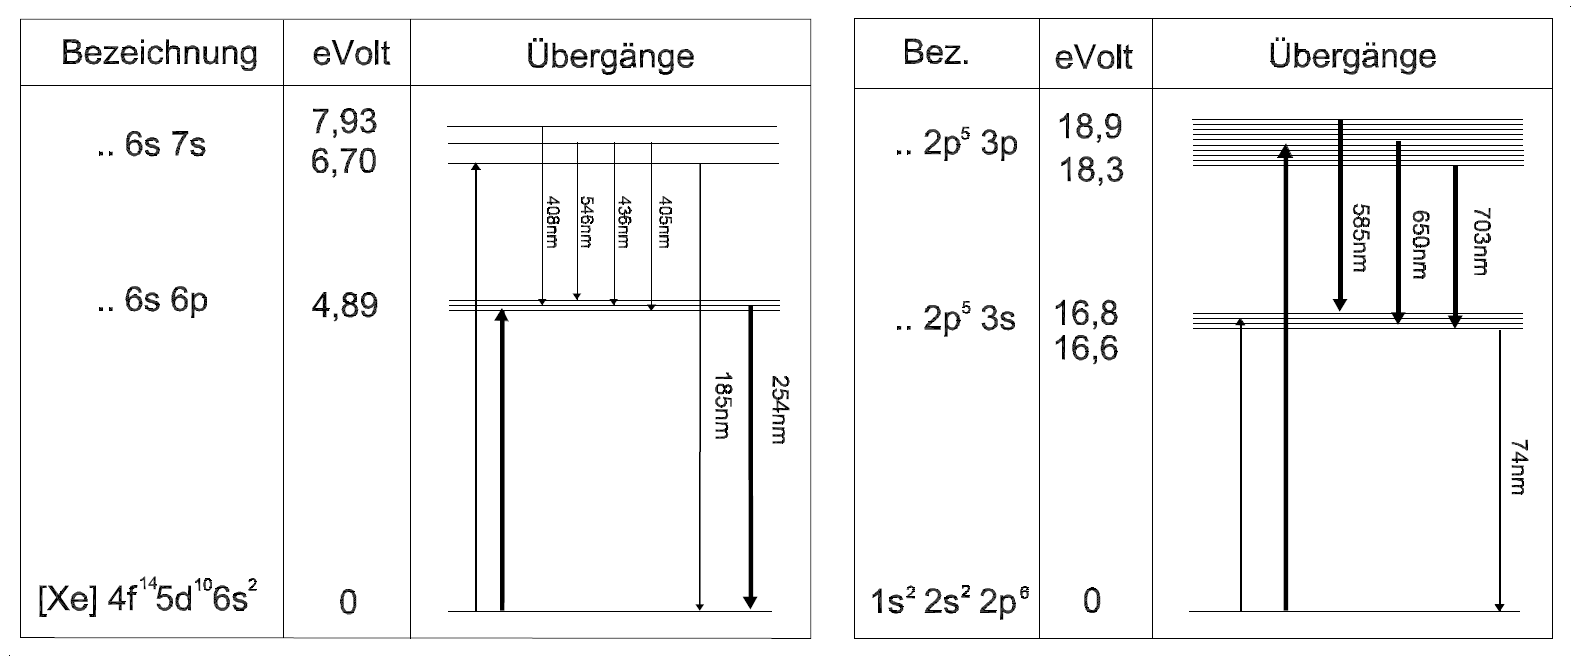
\includegraphics[width=\textwidth]{bilder/Uebergaenge.png}
		\caption{Diese Abbildung stellt das vereinfachte Termschemata von Quecksilber (links) und Neon (rechts) dar. Wahrscheinlichere Übergänge sind mit dickeren Pfeilen hervorgehoben.\cite{WWU}}
		\label{fig:Übergänge}	
	\end{figure}	

		% Charakteristik Ne, Hg(l), Hg(g) 
		% Anregungsspannung bestimmen
		% Angabe Anregungsenergie = eU
		% Wellenlänge
		% Frequenzen der Strahlung
		% Quecksilberdampfdruck nach Clausius
		% mittlere frei Weglänge Hg (l & g)
	% Leuchterscheinungen
	% Quecksilberanregung diesdas
	
	%TODO